% ============================================================
%  methods_draft.tex
%  A STANDALONE draft of the Methods, Results, and Conclusion — NOT the
%  manuscript. Kept separate from main.tex so it can be revised freely.
%
%  It pulls in the auto-generated assets written by
%  scripts/export_paper_assets.py:
%    - figures from  generated/figures/   (white-background PDFs)
%    - tables  from  generated/tables/
%    - numbers from  generated/stats.tex  (macros like \statOverlapMean)
%
%  Compile from inside manuscript/ so the relative paths resolve:
%    pdflatex methods_draft -> bibtex methods_draft -> pdflatex methods_draft x2
% ============================================================
\documentclass[12pt,a4paper]{article}

% ---- Match the manuscript's look ----
\usepackage[T1]{fontenc}
\usepackage[utf8]{inputenc}
\usepackage{newtxtext,newtxmath}            % Times New Roman-like text + math
\usepackage[a4paper,left=2cm,right=2cm,top=2cm,bottom=2cm]{geometry}
\usepackage{setspace}\onehalfspacing
\usepackage{microtype}
\usepackage{amsmath}
\usepackage{graphicx}
\usepackage{booktabs}                        % the generated tables use \toprule etc.
\usepackage[round,authoryear]{natbib}
\usepackage[hidelinks]{hyperref}

% ---- Where to find the generated assets ----
\graphicspath{{generated/figures/}}
% Auto-generated by scripts/export_paper_assets.py — do not edit by hand.
% Each macro is a number quoted in the manuscript; re-run the script to refresh.
% Usage in main.tex:  % Auto-generated by scripts/export_paper_assets.py — do not edit by hand.
% Each macro is a number quoted in the manuscript; re-run the script to refresh.
% Usage in main.tex:  % Auto-generated by scripts/export_paper_assets.py — do not edit by hand.
% Each macro is a number quoted in the manuscript; re-run the script to refresh.
% Usage in main.tex:  \input{generated/stats.tex}   then e.g.  \statOverlapMean

\newcommand{\statNCitiesAnalyzed}{387}
\newcommand{\statOverlapMean}{0.946}
\newcommand{\statOverlapMedian}{0.960}
\newcommand{\statOverlapSkew}{-1.33}
\newcommand{\statOverlapKurt}{1.46}
\newcommand{\statSizePapersR}{+0.71}
\newcommand{\statSizePapersP}{0.000}
\newcommand{\statSizeProjectsR}{+0.70}
\newcommand{\statSizeProjectsP}{0.000}
\newcommand{\statClusterNCitiesAll}{323}
\newcommand{\statClusterMinDocs}{8}
\newcommand{\statClusterNCitiesDense}{60}
\newcommand{\statClusterOlsRsq}{0.064}
\newcommand{\statClusterSizePapersP}{0.066}
\newcommand{\statClusterSizeProjectsP}{0.539}
\newcommand{\statClusterPermObserved}{0.0590}
\newcommand{\statClusterPermNullMean}{0.0390}
\newcommand{\statClusterPermP}{0.0005}
\newcommand{\statClusterPermExcess}{+0.0200}
\newcommand{\statMantelR}{+0.21}
\newcommand{\statMantelP}{0.0010}
\newcommand{\statMantelNCities}{244}
\newcommand{\statNPapersTotal}{10,319}
\newcommand{\statNProjectsTotal}{4,606}
\newcommand{\statPaperYearMin}{2000}
\newcommand{\statPaperYearMax}{2026}
\newcommand{\statProjectYearMin}{2009}
\newcommand{\statProjectYearMax}{2025}
\newcommand{\statAlignMeanDelta}{+0.0135}
\newcommand{\statAlignFracPos}{0.908}
\newcommand{\statAlignT}{77.99}
\newcommand{\statAlignP}{0.0000}
\newcommand{\statAlignNProjects}{3,596}
\newcommand{\statAlignTClustered}{17.70}
\newcommand{\statAlignNCities}{320}
\newcommand{\statAlignDeltaCity}{+0.0084}
\newcommand{\statAlignTCity}{12.19}
\newcommand{\statAlignFracCitiesPos}{0.791}
\newcommand{\statAlignSizeR}{+0.59}
\newcommand{\statAlignSizeP}{0.000}
\newcommand{\statAlignDeltaLarge}{+0.0165}
\newcommand{\statAlignDeltaSmall}{+0.0045}
\newcommand{\statCcAlignN}{111}
\newcommand{\statCcAlignNCities}{79}
\newcommand{\statCcAlignMeanDelta}{+0.0140}
\newcommand{\statCcAlignFracPos}{0.901}
\newcommand{\statCcAlignTClustered}{9.50}
\newcommand{\statDidEstimate}{+0.0026}
\newcommand{\statDidT}{7.33}
\newcommand{\statDidP}{0.0000}
\newcommand{\statDidN}{1,834}
\newcommand{\statDidTClustered}{4.06}
\newcommand{\statDidNCities}{161}
\newcommand{\statLeadlagBestLag}{+3}
\newcommand{\statLeadlagBestSim}{0.9003}
\newcommand{\statNCitiesParts}{348}
\newcommand{\statPartEntropyMedian}{1.557}
\newcommand{\statPartEntropyMax}{3.584}
   then e.g.  \statOverlapMean

\newcommand{\statNCitiesAnalyzed}{387}
\newcommand{\statOverlapMean}{0.946}
\newcommand{\statOverlapMedian}{0.960}
\newcommand{\statOverlapSkew}{-1.33}
\newcommand{\statOverlapKurt}{1.46}
\newcommand{\statSizePapersR}{+0.71}
\newcommand{\statSizePapersP}{0.000}
\newcommand{\statSizeProjectsR}{+0.70}
\newcommand{\statSizeProjectsP}{0.000}
\newcommand{\statClusterNCitiesAll}{323}
\newcommand{\statClusterMinDocs}{8}
\newcommand{\statClusterNCitiesDense}{60}
\newcommand{\statClusterOlsRsq}{0.064}
\newcommand{\statClusterSizePapersP}{0.066}
\newcommand{\statClusterSizeProjectsP}{0.539}
\newcommand{\statClusterPermObserved}{0.0590}
\newcommand{\statClusterPermNullMean}{0.0390}
\newcommand{\statClusterPermP}{0.0005}
\newcommand{\statClusterPermExcess}{+0.0200}
\newcommand{\statMantelR}{+0.21}
\newcommand{\statMantelP}{0.0010}
\newcommand{\statMantelNCities}{244}
\newcommand{\statNPapersTotal}{10,319}
\newcommand{\statNProjectsTotal}{4,606}
\newcommand{\statPaperYearMin}{2000}
\newcommand{\statPaperYearMax}{2026}
\newcommand{\statProjectYearMin}{2009}
\newcommand{\statProjectYearMax}{2025}
\newcommand{\statAlignMeanDelta}{+0.0135}
\newcommand{\statAlignFracPos}{0.908}
\newcommand{\statAlignT}{77.99}
\newcommand{\statAlignP}{0.0000}
\newcommand{\statAlignNProjects}{3,596}
\newcommand{\statAlignTClustered}{17.70}
\newcommand{\statAlignNCities}{320}
\newcommand{\statAlignDeltaCity}{+0.0084}
\newcommand{\statAlignTCity}{12.19}
\newcommand{\statAlignFracCitiesPos}{0.791}
\newcommand{\statAlignSizeR}{+0.59}
\newcommand{\statAlignSizeP}{0.000}
\newcommand{\statAlignDeltaLarge}{+0.0165}
\newcommand{\statAlignDeltaSmall}{+0.0045}
\newcommand{\statCcAlignN}{111}
\newcommand{\statCcAlignNCities}{79}
\newcommand{\statCcAlignMeanDelta}{+0.0140}
\newcommand{\statCcAlignFracPos}{0.901}
\newcommand{\statCcAlignTClustered}{9.50}
\newcommand{\statDidEstimate}{+0.0026}
\newcommand{\statDidT}{7.33}
\newcommand{\statDidP}{0.0000}
\newcommand{\statDidN}{1,834}
\newcommand{\statDidTClustered}{4.06}
\newcommand{\statDidNCities}{161}
\newcommand{\statLeadlagBestLag}{+3}
\newcommand{\statLeadlagBestSim}{0.9003}
\newcommand{\statNCitiesParts}{348}
\newcommand{\statPartEntropyMedian}{1.557}
\newcommand{\statPartEntropyMax}{3.584}
   then e.g.  \statOverlapMean

\newcommand{\statNCitiesAnalyzed}{387}
\newcommand{\statOverlapMean}{0.946}
\newcommand{\statOverlapMedian}{0.960}
\newcommand{\statOverlapSkew}{-1.33}
\newcommand{\statOverlapKurt}{1.46}
\newcommand{\statSizePapersR}{+0.71}
\newcommand{\statSizePapersP}{0.000}
\newcommand{\statSizeProjectsR}{+0.70}
\newcommand{\statSizeProjectsP}{0.000}
\newcommand{\statClusterNCitiesAll}{323}
\newcommand{\statClusterMinDocs}{8}
\newcommand{\statClusterNCitiesDense}{60}
\newcommand{\statClusterOlsRsq}{0.064}
\newcommand{\statClusterSizePapersP}{0.066}
\newcommand{\statClusterSizeProjectsP}{0.539}
\newcommand{\statClusterPermObserved}{0.0590}
\newcommand{\statClusterPermNullMean}{0.0390}
\newcommand{\statClusterPermP}{0.0005}
\newcommand{\statClusterPermExcess}{+0.0200}
\newcommand{\statMantelR}{+0.21}
\newcommand{\statMantelP}{0.0010}
\newcommand{\statMantelNCities}{244}
\newcommand{\statNPapersTotal}{10,319}
\newcommand{\statNProjectsTotal}{4,606}
\newcommand{\statPaperYearMin}{2000}
\newcommand{\statPaperYearMax}{2026}
\newcommand{\statProjectYearMin}{2009}
\newcommand{\statProjectYearMax}{2025}
\newcommand{\statAlignMeanDelta}{+0.0135}
\newcommand{\statAlignFracPos}{0.908}
\newcommand{\statAlignT}{77.99}
\newcommand{\statAlignP}{0.0000}
\newcommand{\statAlignNProjects}{3,596}
\newcommand{\statAlignTClustered}{17.70}
\newcommand{\statAlignNCities}{320}
\newcommand{\statAlignDeltaCity}{+0.0084}
\newcommand{\statAlignTCity}{12.19}
\newcommand{\statAlignFracCitiesPos}{0.791}
\newcommand{\statAlignSizeR}{+0.59}
\newcommand{\statAlignSizeP}{0.000}
\newcommand{\statAlignDeltaLarge}{+0.0165}
\newcommand{\statAlignDeltaSmall}{+0.0045}
\newcommand{\statCcAlignN}{111}
\newcommand{\statCcAlignNCities}{79}
\newcommand{\statCcAlignMeanDelta}{+0.0140}
\newcommand{\statCcAlignFracPos}{0.901}
\newcommand{\statCcAlignTClustered}{9.50}
\newcommand{\statDidEstimate}{+0.0026}
\newcommand{\statDidT}{7.33}
\newcommand{\statDidP}{0.0000}
\newcommand{\statDidN}{1,834}
\newcommand{\statDidTClustered}{4.06}
\newcommand{\statDidNCities}{161}
\newcommand{\statLeadlagBestLag}{+3}
\newcommand{\statLeadlagBestSim}{0.9003}
\newcommand{\statNCitiesParts}{348}
\newcommand{\statPartEntropyMedian}{1.557}
\newcommand{\statPartEntropyMax}{3.584}
                  % defines \statOverlapMean, \statNCitiesAnalyzed, ...

\title{Methods and Results (Draft)}
\date{}

\begin{document}
\maketitle

% ============================================================
\section{Methods}
% ============================================================

This project asks whether the student synthetic biology projects produced in a
city sit in the same neighbourhood of meaning as that city's academic papers.
To answer it we need three things: a corpus of artifacts tied to cities, a way
to turn their text into something a computer can compare, and a set of measures
that capture ``relatedness'' without overstating what it implies. This section
builds those three pieces in order, and shows what each one produces along the
way. Throughout, we are careful to talk about \textit{semantic relatedness} and
\textit{association} rather than cause and effect; the artifacts we compare are
shaped by many shared local factors, and our measures cannot separate a genuine
flow of ideas from a university simply hosting both kinds of work at once.

% ------------------------------------------------------------
\subsection{Data}
% ------------------------------------------------------------

We assemble three kinds of artifact, all carrying a title, an abstract-like
block of text, a year, and a city.

\textbf{iGEM projects.} Every iGEM team documents its project on a public
``wiki'', a webpage that functions much like the abstract of a research paper.
We collected \statNProjectsTotal{} of these projects, spanning
\statProjectYearMin{}--\statProjectYearMax{}, and treat each project's text as
one document. iGEM has been described elsewhere as a well-structured dataset for
studying team-level innovation \citep{santoliniIGEMModelSystem2023}.

\textbf{Academic papers.} We drew synthetic biology papers from OpenAlex, an
open bibliographic database, keeping \statNPapersTotal{} papers from
\statPaperYearMin{}--\statPaperYearMax{}. Each paper contributes its title and
abstract.

\textbf{BioBrick parts.} Every team registers the standardised genetic parts it
used or built. These ``biobricks'' snap together like LEGO bricks, each one
performing a single function in a genetic circuit (a promoter that switches a
gene on, a reporter that produces a measurable signal, and so on). Parts do not
carry a city of their own, but every part was registered by a team, and every
team has a city, so we recover each part's city through its team.

\textbf{Geocoding.} Placing a team in a city is the hardest part of the
pipeline. Team names are often acronyms, and institutions move and rename. We
geocoded in stages: an exact match against the OpenAlex and ROR institution
registries where possible, falling back to lightweight name extraction with a
language model and a final lookup against OpenStreetMap's Nominatim service.

A city only enters our analysis once it has both papers and projects, since the
whole question is about how the two relate. After this filter we are left with
\statNCitiesAnalyzed{} cities. Figure~\ref{fig:activity} shows how the two
corpora grow over time: papers accumulate steadily across the whole period,
while iGEM projects appear only from 2009 onward, when the competition's
documentation became consistent.

\begin{figure}[htbp]
  \centering
  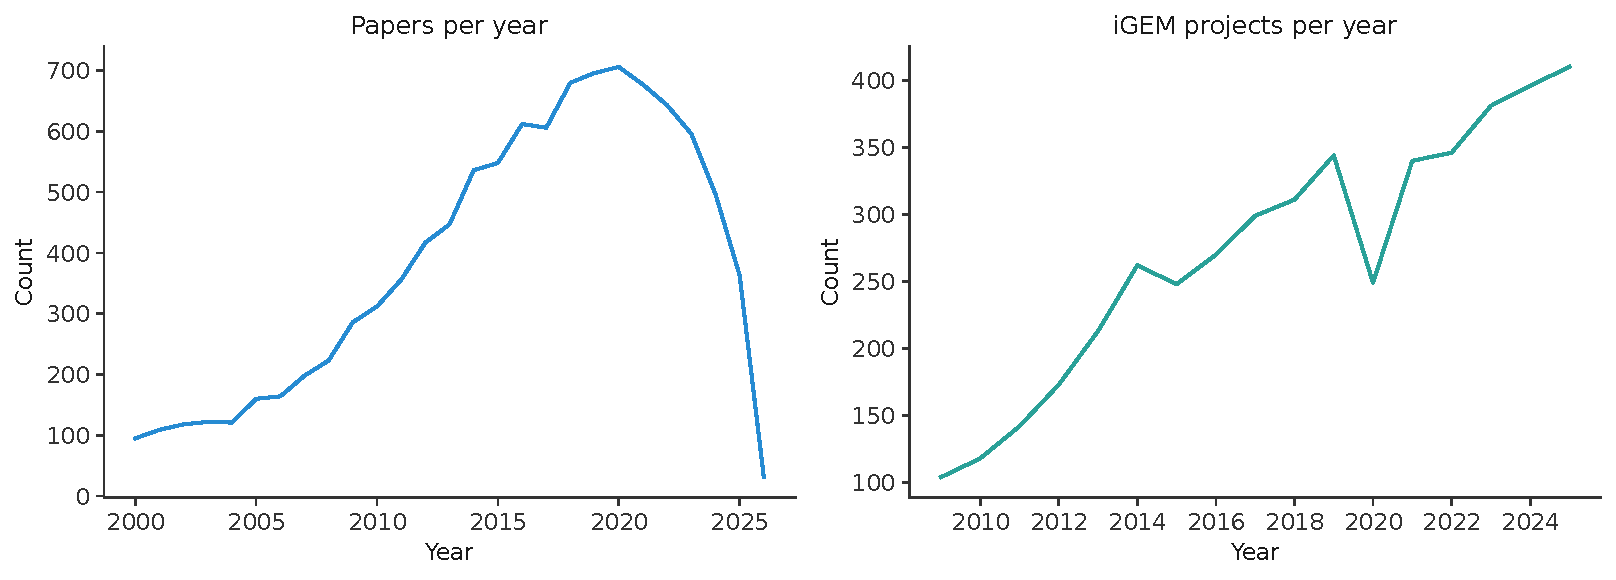
\includegraphics[width=\linewidth]{activity_by_year}
  \caption{Yearly volume of papers (left) and iGEM projects (right). The two
  artifact types cover overlapping but not identical periods, which constrains
  the temporal analysis later in this section.}
  \label{fig:activity}
\end{figure}

% ------------------------------------------------------------
\subsection{Semantic Embeddings}
% ------------------------------------------------------------

To compare text empirically, we need to turn each document into something we can
measure distances between. We do this by building a \textit{semantic embedding
space}: a high-dimensional space in which every document becomes a point, and in
which documents about similar things land close together.

We generate these points with SPECTER2, a natural language model from the Allen
Institute and the successor to the original SPECTER
\citep{cohanDocumentlevelRepresentation2020}.\footnote{SPECTER2 model and
``proximity'' adapter: \url{https://huggingface.co/allenai/specter2}.} SPECTER
belongs to the BERT family of language models \citep{devlinBERTPretrainingDeep2019},
but unlike a general-purpose model it was trained specifically on scientific
papers and their citation graph: it learns to place two documents close together
exactly when one is likely to cite the other. That makes it a natural fit for
our task, where ``related'' is precisely the quantity we are trying to capture.
Each document becomes a 768-dimensional vector.

We chose embeddings over the two obvious alternatives, keyword overlap and
citations, for the same reason. Keyword counting is fragile in synthetic
biology, whose vocabulary overlaps heavily with descriptive molecular biology
\citep{oldhamSyntheticBiologyMapping2018}, so two documents can share words
without sharing meaning, or share meaning while using different words. Citations,
meanwhile, barely exist for student projects. Embeddings sidestep both problems
by working from meaning rather than surface form.

Because SPECTER2 returns unit-length vectors, the natural measure of relatedness
between two documents is the cosine of the angle between them: the closer two
documents point in the same direction, the more semantically related they are.
We use this cosine similarity as the building block for every measure below.

% ------------------------------------------------------------
\subsection{Representing Cities as Centroids}
% ------------------------------------------------------------

A city is not a single document but a cloud of them. To compare cities, we
summarise each cloud by its \textbf{centroid} --- the average of all its
document vectors, re-scaled back to unit length. A city therefore gets two
centroids, one for its papers and one for its projects, each a coarse-grained
``centre of mass'' of that city's work in semantic space.

We then define a city's \textbf{semantic overlap} as the cosine similarity
between its paper centroid and its project centroid. Averaging first and
comparing afterwards is not only faster than comparing every paper to every
project; for unit-length vectors it gives the same answer as the average of all
those pairwise comparisons, which is why centroid-based similarity is a standard
shortcut (Turney \& Pantel, 2010). The idea of summarising a place by the
position of its activity, and reading relatedness off how those positions line
up, follows a long line of work on regional capabilities and the product space
\citep{hidalgoProductSpaceConditions2007, boschmaScientificKnowledgeDynamics2014}.

Figure~\ref{fig:overlap} shows how this measure is distributed across our
\statNCitiesAnalyzed{} cities. Overlap is high and left-skewed, with a mean of
\statOverlapMean{} and a median of \statOverlapMedian{}: most cities sit very
close to 1.0, with a thin tail of low-overlap cities pulling the average down.
The QQ plot confirms the departure from normality (skewness
\statOverlapSkew{}), which matters for any later modelling that assumes
well-behaved errors. Table~\ref{tab:summary} reports the full summary
statistics, and Table~\ref{tab:top15} lists the highest-overlap cities --- all
large, established research hubs with long iGEM histories.

\begin{figure}[htbp]
  \centering
  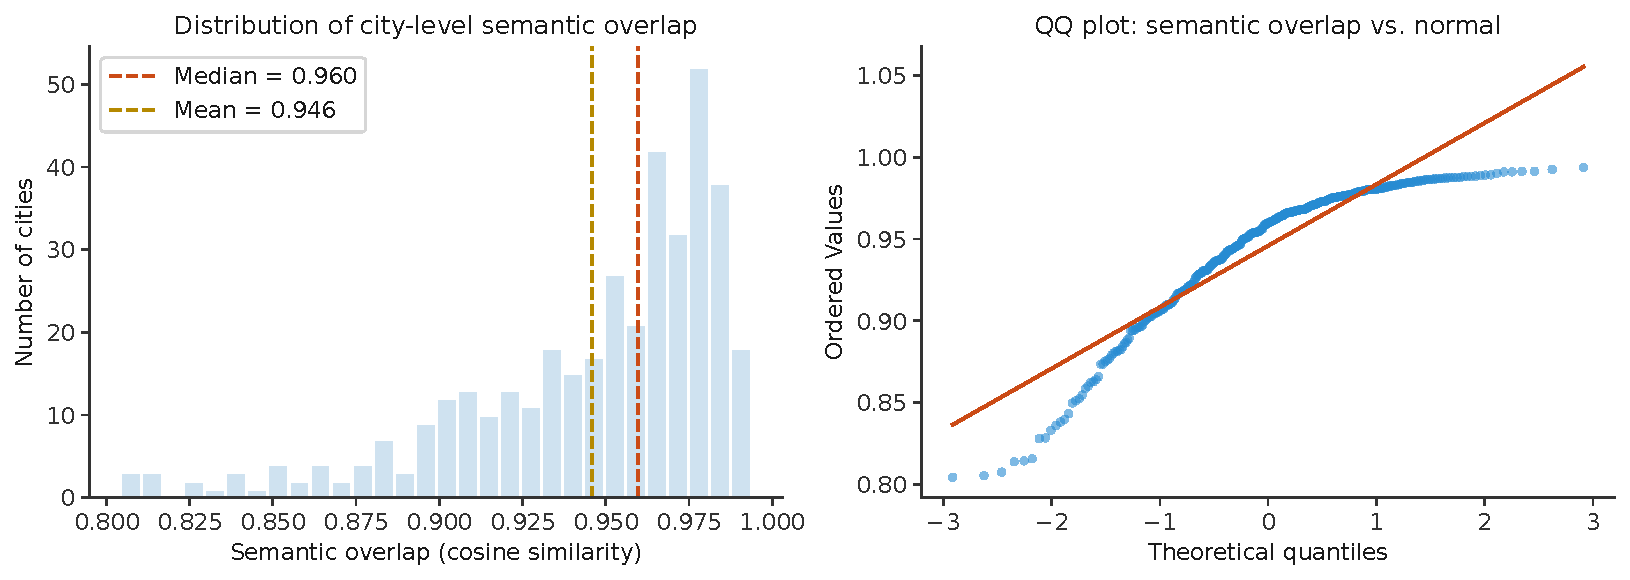
\includegraphics[width=\linewidth]{overlap_distribution}
  \caption{Distribution of city-level semantic overlap (left) and a QQ plot
  against the normal distribution (right). Overlap clusters near 1.0 because all
  documents belong to the same broad field; the spread that remains is what the
  rest of the analysis tries to explain.}
  \label{fig:overlap}
\end{figure}

% Auto-generated by scripts/export_paper_assets.py — do not edit by hand.
\begin{table}[htbp]
\centering
\caption{Summary statistics for the city-level dataset.}
\label{tab:summary}
\begin{tabular}{lrrrrrr}
\toprule
statistic & semantic\_overlap & n\_papers & n\_projects & cs\_paper\_share & cs\_project\_share & proj\_year\_span \\
\midrule
count & 387.000 & 387.000 & 387.000 & 387.000 & 387.000 & 387.000 \\
mean & 0.946 & 20.850 & 9.928 & 0.034 & 0.042 & 7.049 \\
std & 0.040 & 36.471 & 20.626 & 0.103 & 0.126 & 5.749 \\
min & 0.804 & 1.000 & 1.000 & 0.000 & 0.000 & 0.000 \\
25\% & 0.926 & 4.000 & 2.000 & 0.000 & 0.000 & 1.000 \\
50\% & 0.960 & 10.000 & 5.000 & 0.000 & 0.000 & 7.000 \\
75\% & 0.976 & 22.000 & 11.000 & 0.022 & 0.000 & 12.000 \\
max & 0.994 & 364.000 & 258.000 & 1.000 & 1.000 & 16.000 \\
\bottomrule
\end{tabular}

\end{table}

% Auto-generated by scripts/export_paper_assets.py — do not edit by hand.
\begin{table}[htbp]
\centering
\caption{Top 15 cities by semantic overlap.}
\label{tab:top15}
\begin{tabular}{llrrr}
\toprule
city & country & n\_papers & n\_projects & semantic\_overlap \\
\midrule
Cambridge & US & 364 & 40 & 0.994 \\
Shanghai & CN & 126 & 216 & 0.993 \\
Tianjin & CN & 112 & 35 & 0.991 \\
Berkeley & US & 98 & 13 & 0.991 \\
Beijing & CN & 356 & 258 & 0.991 \\
Boston & US & 95 & 25 & 0.991 \\
Hangzhou & CN & 60 & 45 & 0.990 \\
Wuhan & CN & 64 & 102 & 0.989 \\
Changsha & CN & 22 & 26 & 0.989 \\
Urbana & US & 60 & 16 & 0.989 \\
Marburg & DE & 32 & 11 & 0.989 \\
Munich & DE & 58 & 18 & 0.988 \\
Paris & FR & 147 & 37 & 0.988 \\
Guangzhou & CN & 63 & 52 & 0.988 \\
Xiamen & CN & 11 & 21 & 0.988 \\
\bottomrule
\end{tabular}

\end{table}

That high baseline is also a warning. Because every document in the corpus is
synthetic biology, any two city centroids start out fairly close simply by
belonging to the same field, and larger cities --- with more documents averaged
into each centroid --- tend to have steadier, more representative centres.
Figure~\ref{fig:size} makes this concrete: semantic overlap rises with the
number of papers ($r = \statSizePapersR{}$) and projects
($r = \statSizeProjectsR{}$) a city has. This is the familiar tension between
diversity and relatedness in regional science, and it means we cannot read raw
overlap as evidence of local idea flow on its own. The measures in the next
three subsections are designed to look past this baseline.

\begin{figure}[htbp]
  \centering
  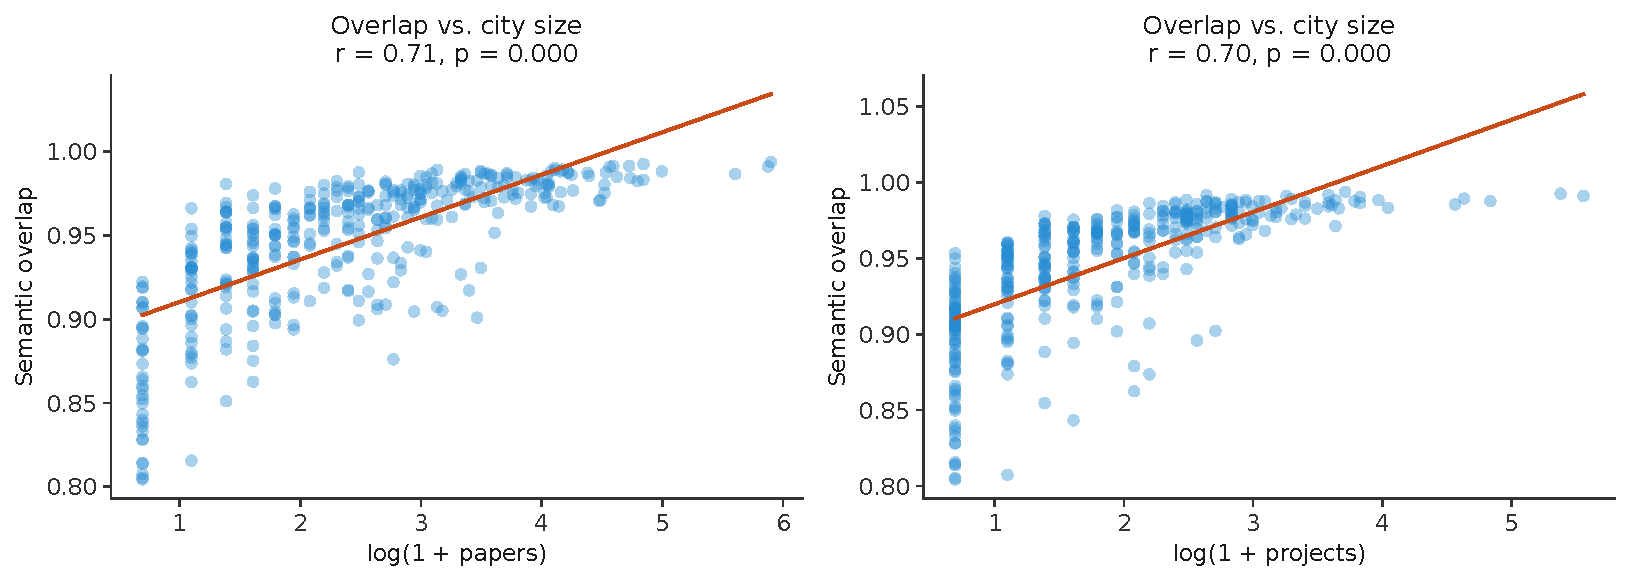
\includegraphics[width=\linewidth]{overlap_vs_size}
  \caption{Semantic overlap against city size, measured by paper count (left)
  and project count (right) on a log scale. Both relationships are strongly
  positive, so part of a city's overlap reflects how much it produces rather
  than how aligned its two outputs are.}
  \label{fig:size}
\end{figure}

% ------------------------------------------------------------
\subsection{Local Alignment: Is a Project Closer to Its Own City?}
% ------------------------------------------------------------

Instead of comparing the two centroids of a single city, we can ask a sharper
question one project at a time: is an individual iGEM project more similar to its
\textit{own} city's papers than to the papers of every other city? If projects
and papers really share local roots, the answer should be yes.

For each project we compute its cosine similarity to its home city's paper
centroid, and its average similarity to the paper centroids of all other cities
(keeping only cities with at least three papers, so the centroids are stable).
The difference between the two, which we call $\delta$, is positive whenever a
project looks more like home than like elsewhere. Across \statAlignNProjects{}
projects the mean advantage is $\delta = \statAlignMeanDelta{}$, and
\statAlignFracPos{} of projects are individually positive
($t = \statAlignT{}$, $p < 0.001$). Figure~\ref{fig:align} shows the full
distribution and the project-by-project comparison.

The effect is small in absolute terms --- a consequence of the same field-level
baseline noted above --- but it is consistent: projects do sit nearer their own
city's research than a random city's. We read this as evidence of local
\textit{relatedness}, not of any causal pull, since a shared university faculty
could easily produce both kinds of work on the same theme without one feeding
the other.

\begin{figure}[htbp]
  \centering
  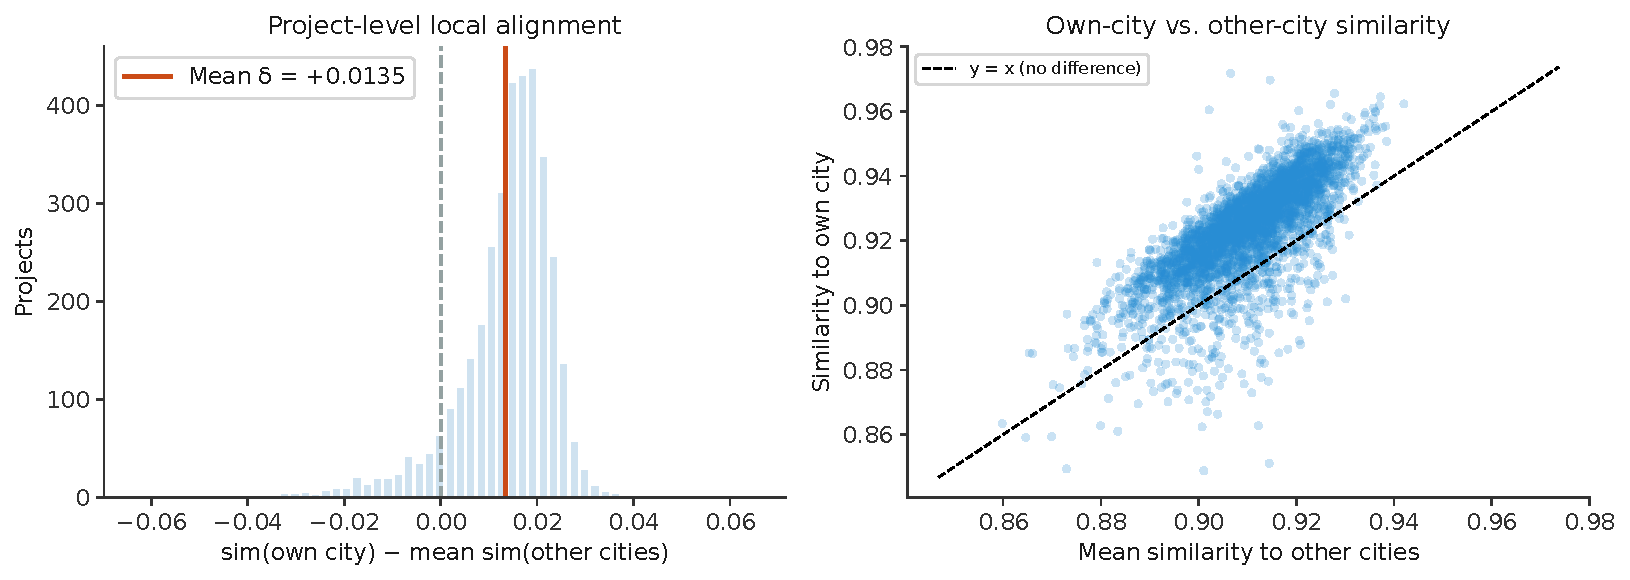
\includegraphics[width=\linewidth]{project_level_alignment}
  \caption{Local alignment at the project level. Left: the distribution of
  $\delta$, each project's similarity to its own city's papers minus its mean
  similarity to other cities' papers; mass to the right of zero indicates local
  alignment. Right: own-city versus other-city similarity, where points above
  the diagonal are the locally aligned projects.}
  \label{fig:align}
\end{figure}

% ------------------------------------------------------------
\subsection{Stable Specialisation versus Local Timing: A Difference-in-Differences Design}
% ------------------------------------------------------------

The local advantage in the previous test could mean two quite different things.
It might reflect a genuine, time-specific connection --- this year's projects
tracking this year's local papers. Or it might just reflect a city's stable
identity: a place that has always worked on biosensors will have both projects
and papers about biosensors in every year, with no idea flowing between them at
all. To separate these, we borrow the logic of a \textbf{difference-in-differences}
design, the workhorse of applied econometrics (Angrist \& Pischke, 2009).

The idea is a two-by-two comparison. For each project we measure its similarity
to its own city's papers and to other cities' papers, and we do this both in the
project's \textit{own year} and in \textit{other years}. A stable-specialisation
story predicts a home-city advantage even in other years; a local-timing story
predicts an \textit{extra} advantage in the project's own year, on top of that.
The difference-in-differences is exactly that extra slice. Table~\ref{tab:did}
reports the four cells, and Figure~\ref{fig:did} shows them alongside the
distribution of the per-project estimate.

% Auto-generated by scripts/export_paper_assets.py — do not edit by hand.
\begin{table}[htbp]
\centering
\caption{Difference-in-differences cells: mean cosine similarity between iGEM projects and annual paper centroids.}
\label{tab:did}
\begin{tabular}{lrr}
\toprule
 & Own city & Other cities \\
\midrule
Own year & 0.9125 & 0.8990 \\
Other years & 0.9063 & 0.8954 \\
\bottomrule
\end{tabular}

\end{table}

Across \statDidN{} projects the estimate is positive and statistically
detectable ($\text{DiD} = \statDidEstimate{}$, $t = \statDidT{}$,
$p < 0.001$), but it is tiny next to the stable-specialisation gap that sits
underneath it. In plain terms: most of why a project resembles its city's papers
is that the city has a durable thematic identity, with only a sliver attributable
to same-year alignment. This is a useful corrective to a naive reading of the
local-alignment result.

\begin{figure}[htbp]
  \centering
  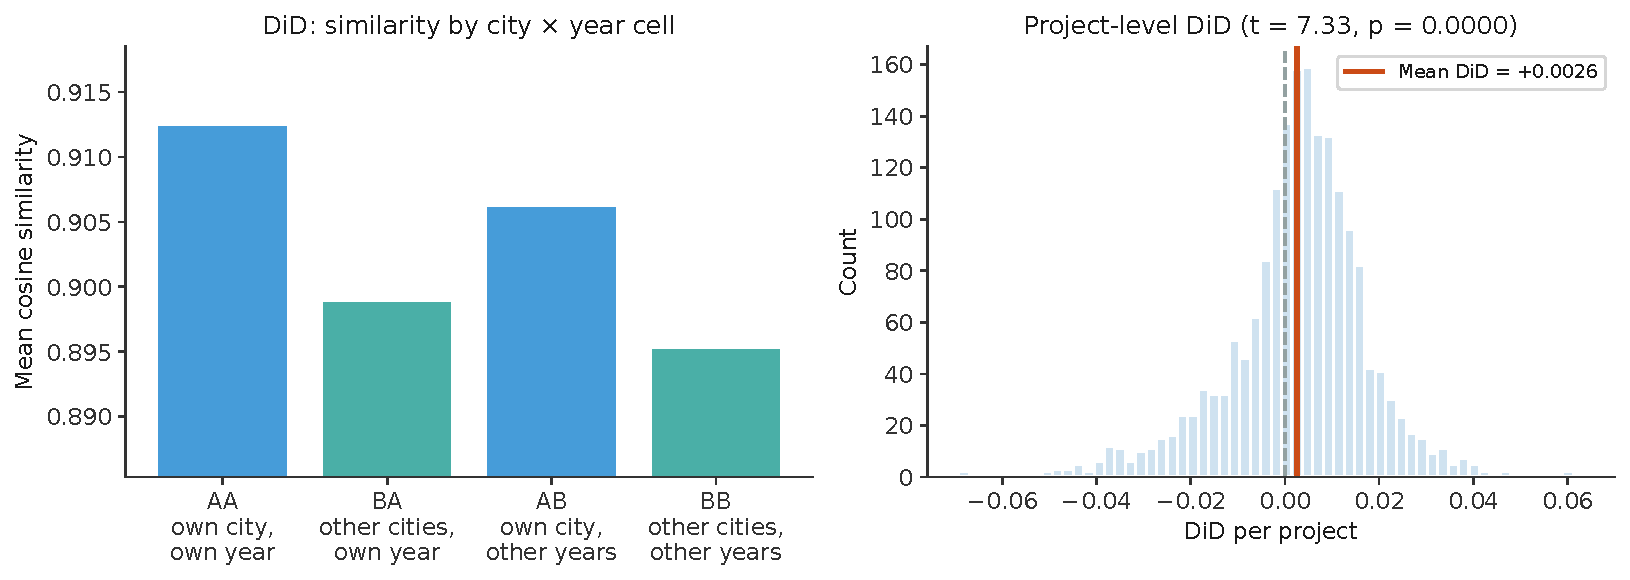
\includegraphics[width=\linewidth]{did_alignment}
  \caption{Difference-in-differences. Left: mean similarity in each of the four
  city\,$\times$\,year cells. Right: the distribution of the per-project
  difference-in-differences; its small positive mean is the part of local
  alignment that is specific to the project's own year.}
  \label{fig:did}
\end{figure}

% ------------------------------------------------------------
\subsection{Temporal Structure: Do Projects Lead Papers?}
% ------------------------------------------------------------

The guiding intuition of this thesis is that student projects might introduce
early ideas that academic papers later develop. If so, a city's projects in year
$t$ should look most like its papers a few years \textit{after} $t$. To test the
shape of this relationship we build annual centroids for each city's projects and
papers, and for every project-year we record its similarity to the city's paper
centroid at offsets from three years before to three years after. Averaging over
all city-years gives a \textbf{lead--lag profile}: similarity as a function of
the offset $k$, where positive $k$ means papers come after projects. This is the
descriptive, correlational cousin of a Granger lead--lag analysis (Granger,
1969); we use it to describe timing, not to claim causation.

Figure~\ref{fig:leadlag} and Table~\ref{tab:leadlag} show the result, and the
honest summary is that the profile is nearly flat. The nominal peak sits at
$k = \statLeadlagBestLag{}$ (mean similarity \statLeadlagBestSim{}), which would
be consistent with projects leading papers, but the difference across the whole
range is on the order of a thousandth of a cosine unit and the confidence
intervals overlap almost everywhere. Our reading is that city-level annual
centroids are simply too coarse --- often built from a single document in a given
year --- to resolve a lead--lag signal if one exists. We report the test because
the null result is informative about the method, not because it settles the
question.

% Auto-generated by scripts/export_paper_assets.py — do not edit by hand.
\begin{table}[htbp]
\centering
\caption{Lead-lag similarity profile between project and paper centroids.}
\label{tab:leadlag}
\begin{tabular}{rrrrr}
\toprule
lag & n\_pairs & mean\_sim & ci\_lo & ci\_hi \\
\midrule
-3 & 1253 & 0.8950 & 0.8927 & 0.8972 \\
-2 & 1300 & 0.8966 & 0.8946 & 0.8988 \\
-1 & 1357 & 0.8975 & 0.8952 & 0.8997 \\
0 & 1383 & 0.8988 & 0.8966 & 0.9008 \\
1 & 1324 & 0.9000 & 0.8979 & 0.9020 \\
2 & 1270 & 0.8997 & 0.8975 & 0.9019 \\
3 & 1189 & 0.9003 & 0.8981 & 0.9025 \\
\bottomrule
\end{tabular}

\end{table}

\begin{figure}[htbp]
  \centering
  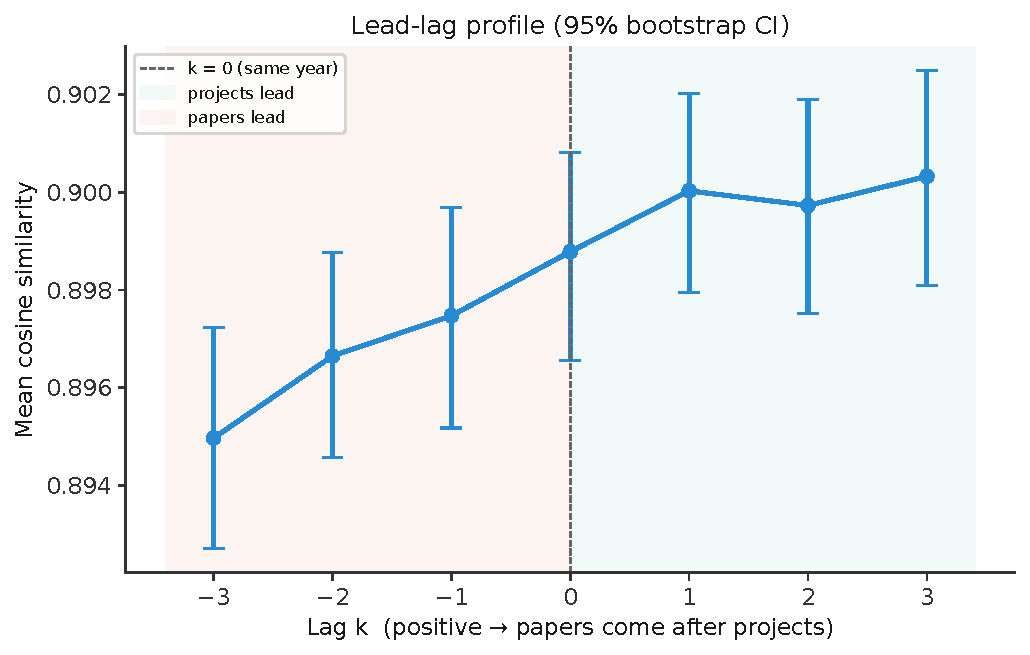
\includegraphics[width=0.72\linewidth]{lead_lag_profile}
  \caption{Lead--lag profile between project and paper centroids, with 95\%
  bootstrap confidence intervals. Positive lags mean papers follow projects. The
  profile is close to flat, so the data neither confirm nor rule out the
  early-signal hypothesis.}
  \label{fig:leadlag}
\end{figure}

% ------------------------------------------------------------
\subsection{Beyond Text: BioBrick Part-Type Composition}
% ------------------------------------------------------------

Everything so far rests on text. As an independent check, we turn to the
physical parts each city's teams actually registered. The \textit{mix} of part
types a city deposits --- coding sequences, regulatory elements, reporters, and
so on --- is a fingerprint of the kind of biology it does, and it is measured
completely separately from the embedding space. If our text-based picture is
capturing something real, the two should broadly agree.

For each city with at least ten registered parts (\statNCitiesParts{} cities in
all) we compute the share of its parts in each functional category, and summarise
how specialised that mix is with its Shannon entropy: low entropy means a city
concentrates on one type of part, high entropy means it spreads across many. The
median city sits at \statPartEntropyMedian{} nats, well below the
\statPartEntropyMax{} nats a perfectly even spread would give, so cities do tend
to specialise. Figure~\ref{fig:parts} shows the spread of specialisation and the
part-type fingerprints of the most active cities.

\begin{figure}[htbp]
  \centering
  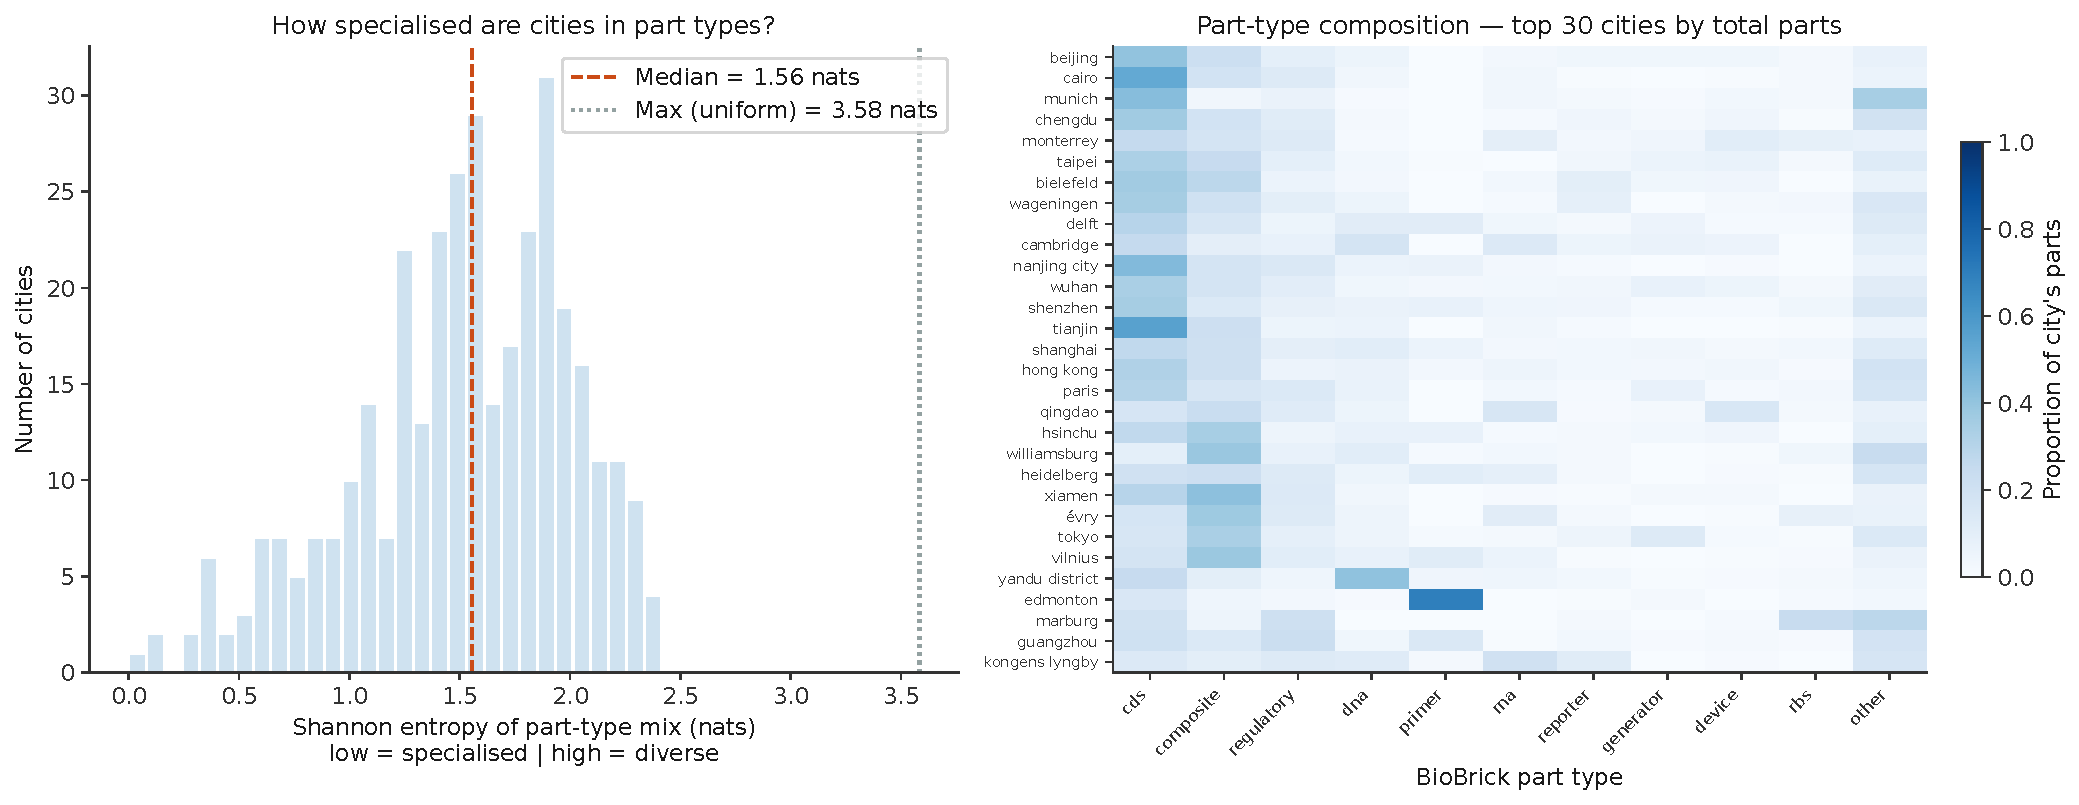
\includegraphics[width=\linewidth]{part_type_composition}
  \caption{BioBrick part-type composition. Left: the distribution of part-type
  entropy across cities; most cities lean toward specialisation. Right: the
  part-type profile of the thirty cities with the most registered parts, sorted
  so that cities with a shared dominant type sit together.}
  \label{fig:parts}
\end{figure}

% ------------------------------------------------------------
\subsection{Interpretive Caution}
% ------------------------------------------------------------

Two limitations shape how far these measures can be pushed, and we flag them here
rather than burying them. First, because the entire corpus is synthetic biology,
cosine similarity between city centroids is dominated by field-level similarity:
two cities look alike mostly because they both do synthetic biology, and only
secondarily because of any genuine local alignment. The difference-in-differences
result makes this concrete, and it is why we lean on the sharper, within-city
comparisons rather than on raw overlap. Second, papers are geocoded to a single
affiliation, so multi-city collaborations are flattened, and our annual centroids
are too thin to support fine temporal claims. Accordingly we frame every result
in this section as semantic relatedness and plausible co-location, and we leave
claims of causal knowledge flow to future work with finer, author- and
mentor-level data.

% ============================================================
\section{Results}
% ============================================================

The Methods section reported each measure's numbers where it built the measure.
Here we step back and read those numbers as three escalating claims, each more
demanding than the last. The first is a sanity check: that the embedding space
recovers a recognisable map of the field at all. The second is the thesis's
central empirical claim: that a city's student projects and its academic papers
occupy related regions of that map. The third is the most ambitious, and the one
we can least support: that the two are linked in time, with projects running
ahead of papers. We take them in turn, then ask whether anything outside the text
agrees.

% ------------------------------------------------------------
\subsection{The Embedding Space Recovers a Sensible Map}
% ------------------------------------------------------------

Before asking whether projects and papers align, we should check that the space
they live in is meaningful. Two features suggest it is. The cities with the
highest project--paper overlap (Table~\ref{tab:top15}) are precisely the places
one would name without any model in hand: Cambridge, Boston and Berkeley in the
United States; Beijing, Shanghai, Tianjin and Wuhan in China; Munich and Marburg
in Germany; Paris in France --- large, long-running synthetic biology hubs with
deep iGEM histories. The cities at the other end (Table~\ref{tab:bottom15}) are
almost all places with a single paper and a single project, where a centroid is
just one document and overlap is whatever that lone pairing happens to be. Low
overlap, in other words, tracks thin data rather than genuine thematic
divergence, exactly as the size relationship ($r = \statSizePapersR{}$ for
papers, $r = \statSizeProjectsR{}$ for projects) leads us to expect. The map
behaves the way a sensible map should: it puts the well-known hubs at the top and
reserves its uncertainty for the cities we know least about.

% Auto-generated by scripts/export_paper_assets.py — do not edit by hand.
\begin{table}[htbp]
\centering
\caption{Bottom 15 cities by semantic overlap.}
\label{tab:bottom15}
\begin{tabular}{llrrr}
\toprule
city & country & n\_papers & n\_projects & semantic\_overlap \\
\midrule
Guwahati & IN & 3 & 1 & 0.851 \\
Santa Clara & US & 1 & 1 & 0.850 \\
Roorkee & IN & 1 & 4 & 0.843 \\
Noda & JP & 1 & 1 & 0.840 \\
Phoenix & US & 1 & 1 & 0.838 \\
Bogor & ID & 1 & 1 & 0.836 \\
Agra & IN & 1 & 1 & 0.833 \\
Merced & US & 1 & 1 & 0.828 \\
León & ES & 1 & 1 & 0.828 \\
Tampa & US & 2 & 1 & 0.816 \\
West Point & US & 1 & 1 & 0.814 \\
Orléans & FR & 1 & 1 & 0.814 \\
Kfar Saba & IL & 1 & 2 & 0.807 \\
Charleston & US & 1 & 1 & 0.805 \\
Boca Raton & US & 1 & 1 & 0.804 \\
\bottomrule
\end{tabular}

\end{table}

% ------------------------------------------------------------
\subsection{Projects and Papers Co-specialise Within Cities}
% ------------------------------------------------------------

The central result is that an iGEM project sits closer to its own city's papers
than to other cities' papers. Across \statAlignNProjects{} projects the mean
advantage is $\delta = \statAlignMeanDelta{}$, and \statAlignFracPos{} of
projects are individually on the home-city side of the line ($t = \statAlignT{}$,
$p < 0.001$). The effect is small in cosine units but extraordinarily consistent
--- roughly nine projects in ten point home --- which is what we would expect if
student work and local research draw on a shared regional base.

But ``closer to home'' can mean two things, and the difference-in-differences
design separates them. Only \statDidEstimate{} of the home-city advantage is
specific to a project's own year (Table~\ref{tab:did}; $t = \statDidT{}$,
$p < 0.001$); the rest is a standing gap that holds in other years too. The
honest reading is that co-specialisation is real and durable but largely
\textit{static}: a city that works on a theme tends to produce both projects and
papers on it across many years, and only a sliver of the alignment reflects
projects and papers moving together year to year. This is a more modest claim
than a knowledge pipeline, and it is the one the data actually support.

% ------------------------------------------------------------
\subsection{Timing Is Unresolved, but the Parts Agree}
% ------------------------------------------------------------

The most ambitious claim --- that projects lead papers --- we cannot make. The
lead--lag profile (Table~\ref{tab:leadlag}, Figure~\ref{fig:leadlag}) rises
gently from lag $-3$ to lag $+3$, with its nominal peak at
$k = \statLeadlagBestLag{}$ years, the direction the early-signal hypothesis
predicts. But the whole profile spans about a thousandth of a cosine unit and the
confidence intervals overlap throughout, so we treat it as flat. City--year
centroids built from a handful of documents are simply too coarse to resolve
timing, and we report the null because it is informative about the method's
limits, not because it settles the question.

What does survive is an independent corroboration from outside the text. The mix
of BioBrick part types a city registers --- measured with no reference to the
embedding space --- shows the same specialisation the text does
(Figure~\ref{fig:parts}): the median city's part-type entropy is
\statPartEntropyMedian{} nats against a possible \statPartEntropyMax{}, so cities
concentrate on particular kinds of biology rather than spreading evenly. That two
methods built on entirely different data --- abstract text on one side,
registered parts on the other --- both point to local specialisation gives us
more confidence that the specialisation lives in the cities, not in the model.

% ============================================================
\section{Conclusion}
% ============================================================

The question this draft set out to answer was whether cities that host student
synthetic biology projects also produce academic papers in related areas. The
answer is a qualified yes. A city's iGEM projects sit measurably nearer its own
papers than other cities' papers, the pattern holds across roughly nine of every
ten projects, and it is echoed by a parts-based fingerprint that never touches
the embedding model. Cities do appear to specialise, and their student and
academic work specialises together.

Two qualifications keep that finding honest. First, the alignment is mostly a
stable feature of a city's identity rather than a year-by-year coupling: the
difference-in-differences result shows that the same-year, ``this project tracks
this paper'' component is real but small. We therefore describe a \textit{local
innovation trajectory} as shared standing specialisation, not as a demonstrated
flow of ideas from students to scholars. Second, our strongest temporal
hypothesis --- that projects run ahead of papers --- is neither confirmed nor
refuted; the city--year centroids are too thin to resolve it, and saying so
plainly is part of the result. Both qualifications echo the interpretive caution
above: with a corpus that is entirely synthetic biology, field-level similarity
sets a high baseline, and the signal we care about lives in the small margins on
top of it.

These limits also point the way forward. The clearest gains would come from finer
links than centroids can provide: scraping the DOIs that iGEM teams cite on their
wikis, to build a direct citation network between projects and the local
literature; matching paper, patent, and team authors to ask whether researchers
stay in the orbit of their old iGEM collaborators; and matching BioBrick
sequences to patent filings through sequence databases, to trace individual
pieces of genetic code from an open registry into commercial application. Each
would replace a coarse, centroid-level association with a concrete, traceable
link --- and would let a future study ask not just whether a city's projects and
papers are related, but whether one actually grew out of the other.

\bibliographystyle{plainnat}
\bibliography{references}

\end{document}
